%%%%%%%%%%%%%%%%%%%%%%%%%%%%%%%%%%%%%%%%%
% Template Original author:
% Frits Wenneker (http://www.howtotex.com)
%
% License:
% CC BY-NC-SA 3.0 (http://creativecommons.org/licenses/by-nc-sa/3.0/)
%%%%%%%%%%%%%%%%%%%%%%%%%%%%%%%%%%%%%%%%%

%----------------------------------------------------------------------------------------
%	PACKAGES AND OTHER DOCUMENT CONFIGURATIONS
%----------------------------------------------------------------------------------------

\documentclass[fontsize=11pt]{scrartcl} % A4 paper and 11pt font size

\usepackage[T1]{fontenc} % Use 8-bit encoding that has 256 glyphs
\usepackage{fourier} % Use the Adobe Utopia font for the document - comment this line to return to the LaTeX default
\usepackage[english]{babel} % English language/hyphenation
\usepackage{amsmath,amsfonts,amsthm} % Math packages

\usepackage{lipsum} % Used for inserting dummy 'Lorem ipsum' text into the template

\usepackage{sectsty} % Allows customizing section commands
\allsectionsfont{\centering \normalfont\scshape} % Make all sections centered, the default font and small caps

\usepackage{fancyhdr} % Custom headers and footers
\pagestyle{fancyplain} % Makes all pages in the document conform to the custom headers and footers
\fancyhead{} % No page header - if you want one, create it in the same way as the footers below
\fancyfoot[L]{} % Empty left footer
\fancyfoot[C]{} % Empty center footer
\fancyfoot[R]{\thepage} % Page numbering for right footer
\renewcommand{\headrulewidth}{0pt} % Remove header underlines
\renewcommand{\footrulewidth}{0pt} % Remove footer underlines
\setlength{\headheight}{13.6pt} % Customize the height of the header

\numberwithin{equation}{section} % Number equations within sections (i.e. 1.1, 1.2, 2.1, 2.2 instead of 1, 2, 3, 4)
\numberwithin{figure}{section} % Number figures within sections (i.e. 1.1, 1.2, 2.1, 2.2 instead of 1, 2, 3, 4)
\numberwithin{table}{section} % Number tables within sections (i.e. 1.1, 1.2, 2.1, 2.2 instead of 1, 2, 3, 4)

\setlength\parindent{0pt} % Removes all indentation from paragraphs - comment this line for an assignment with lots of text

\usepackage{tikz}
\tikzset{main node/.style={circle,fill=blue!20,draw,minimum size=1cm,inner sep=0pt},
}
\usetikzlibrary{positioning}

%----------------------------------------------------------------------------------------
%	TITLE SECTION
%----------------------------------------------------------------------------------------

\newcommand{\horrule}[1]{\rule{\linewidth}{#1}} % Create horizontal rule command with 1 argument of height

\title{	
\normalfont \normalsize 
\textsc{George Washington University, Department of Mathematics} \\ [25pt] % Your university, school and/or department name(s)
\textsc{Graph Theory, MATH 3632}
\horrule{0.5pt} \\[0.4cm] % Thin top horizontal rule
\huge Problem Set I (Revisions)\\ % The assignment title
\horrule{2pt} \\[0.5cm] % Thick bottom horizontal rule
}

\author{Joseph Espy} % Your name

\date{\normalsize\today} % Today's date or a custom date

\begin{document}

\maketitle % Print the title

\section*{Exercise II}
	For every $k$-regular graph is there a $(k+1)$-regular graph that contains the $k$-regular graph as a subgraph?\\
	
	There is.  Let $G= (V, E, \phi)$ be any $k$-regular graph.  Let us construct $G_a = (V_a, E_a, \phi_a)$ by relabeling $G$ such that $V(G) \cap V(G_a) = \emptyset$, $E(G) \cap E(G_a) = \emptyset$, and $\phi(G) \cap \phi(G_a) = \emptyset$\\
	
	Because $G_a$ is a relabeling of $G$, it is an isomorphism.  This implies that there exists a bijection $f: V(G)\rightarrow V(G_a)$ which satisfies all of the properties of isomorphism.  \\
	
	Let us consider $G'$ which has $G$ and $G_a$ as subgraphs.  Now add an edge in $G'$ from $v$ to $v'$ for every $v \in V(G), v' \in V(G')$ where $v' = f(v)$.  ($f$ is the isomorphism bijection from above).  \\
	
	The degree of each vertex $v \in V(G')$ is exactly $k+1$.  $V$ has $k$ edges because it is in $V(G)$ or $V(G_a)$ which are both $k$-regular.  It has an additional edge from the bijection which creates exactly one edge per $v \in V(G')$.  So each vertex has degree $k+1$, so the graph $G'$ is $(k+1)$-regular.  So for every $k$-regular graph, there is a $(k+1)$-regular graph that contains the $k$-regular graph as a sub graph.  \qed


\section*{Exercise IV}
			If a simple graph $G$ is isomorphic to its complement $\overline G$, then $G$ has either $4k$ or $4k+1$ vertices for some $k \in \mathbb{N}$.  Find all simple graphs in on four and five vertices that are isomorphic to their complements.\\
			
			Proof that if a simple graph $G$ is isomorphic to its complement $\overline G$, then $G$ has either $4k$ or $4k+1$ vertices for some $k \in \mathbb{N}$.\\
			
			Given a set of $n$ vertices, there are $\frac{n(n+1)}{2}$ edges that a simple graph can have ($\sum_{i=1}^{i=n} i$).  No edge exists in both the graph $G$ and $\overline{G}$, while every edge exists in at least $G$ or $\overline{G}$.  Two graphs which are isomorphic will have the same number of edges.  So a graph which is isomorphic to its complement will have $\frac{n(n-1)}{4}$ edges.  \\
			
			The number of edges must be an integer, so $4|n(n-1)$.  This implies that $4|n$ or $4|n-1$.  From this, a simple graph which is isomorphic to its complement will have $4k$ or $4k+1$ nodes for some integer $k$.  \\
			
			The graphs up to isomorphism on four vertices which is isomorphic to its own complement is $P_4$ (a specific labeling is shown along with the isomorphic complement):
						
			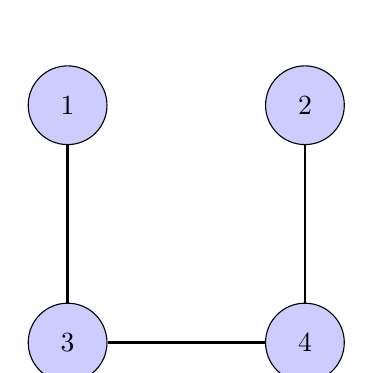
\begin{tikzpicture}
			
			%%
			\begin{scope}[xshift=4cm]
			\node[main node] (1) {$1$};
			\node[main node] (2) [right = 2cm  of 1]  {$2$};
			\node[main node] (3) [below = 2cm  of 1] {$3$};
			\node[main node] (4) [right = 2cm  of 3] {$4$};
			
			\path[draw,thick]
			(1) edge node {} (3)
			(3) edge node {} (4)
			(4) edge node {} (2)
			;
			\end{scope}
			\end{tikzpicture}
			
			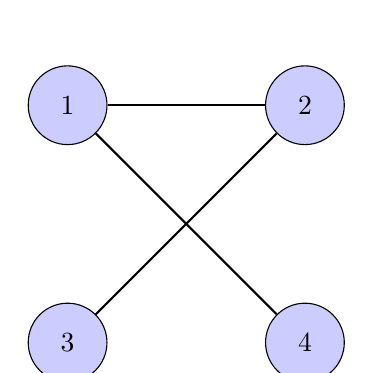
\begin{tikzpicture}
			
			%%
			\begin{scope}[xshift=4cm]
			\node[main node] (1) {$1$};
			\node[main node] (2) [right = 2cm  of 1]  {$2$};
			\node[main node] (3) [below = 2cm  of 1] {$3$};
			\node[main node] (4) [right = 2cm  of 3] {$4$};
			
			\path[draw,thick]
			(1) edge node {} (2)
			(1) edge node {} (4)
			(3) edge node {} (2)
			;
			\end{scope}
			\end{tikzpicture}
			
			The only two graphs up to isomorphism on five vertexes which are isomorphic to their own complements are: (The first is $C_n$, a specific labeling is shown along with its complement)
			
			
			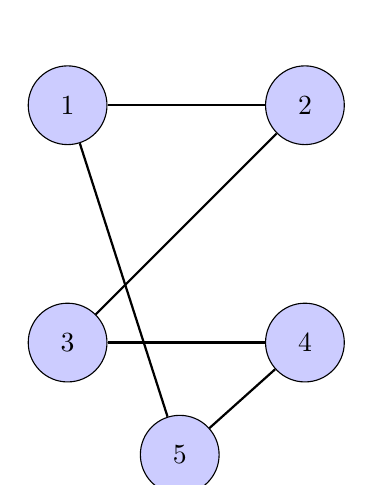
\begin{tikzpicture}
			
			%%
			\begin{scope}[xshift=4cm]
			\node[main node] (1) {$1$};
			\node[main node] (2) [right = 2cm  of 1]  {$2$};
			\node[main node] (3) [below = 2cm  of 1] {$3$};
			\node[main node] (4) [right = 2cm  of 3] {$4$};
			\node[main node] (5) [below right = 1cm  of 3] {$5$};
			
			\path[draw,thick]
			(1) edge node {} (2)
			%(1) edge node {} (3)
			%(1) edge node {} (4)
			(1) edge node {} (5)
			(2) edge node {} (3)
			%(2) edge node {} (4)
			%(2) edge node {} (5)
			(3) edge node {} (4)
			%(3) edge node {} (5)
			(4) edge node {} (5)
			;
			\end{scope}
			\end{tikzpicture}
			
			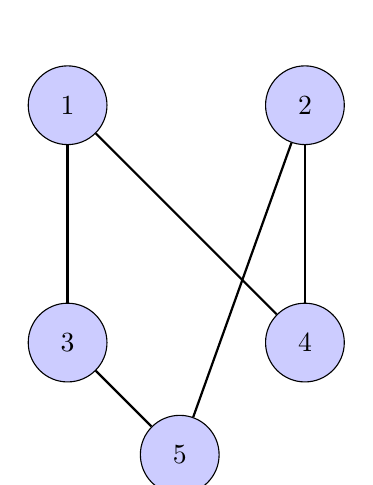
\begin{tikzpicture}
			
			%%
			\begin{scope}[xshift=4cm]
			\node[main node] (1) {$1$};
			\node[main node] (2) [right = 2cm  of 1]  {$2$};
			\node[main node] (3) [below = 2cm  of 1] {$3$};
			\node[main node] (4) [right = 2cm  of 3] {$4$};
			\node[main node] (5) [below right = 1cm  of 3] {$5$};
			
			\path[draw,thick]
			%(1) edge node {} (2)
			(1) edge node {} (3)
			(1) edge node {} (4)
			%(1) edge node {} (5)
			%(2) edge node {} (3)
			(2) edge node {} (4)
			(2) edge node {} (5)
			%(3) edge node {} (4)
			(3) edge node {} (5)
			%(4) edge node {} (5)
			;
			\end{scope}
			\end{tikzpicture}	\\
			
			A labeling for the second isomorphism and its isomorphic complement is:	\\
			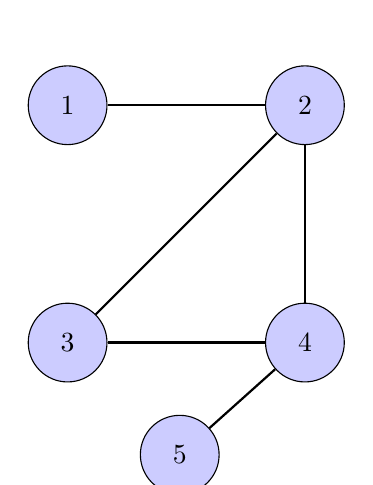
\begin{tikzpicture}
			
			%%
			\begin{scope}[xshift=4cm]
			\node[main node] (1) {$1$};
			\node[main node] (2) [right = 2cm  of 1]  {$2$};
			\node[main node] (3) [below = 2cm  of 1] {$3$};
			\node[main node] (4) [right = 2cm  of 3] {$4$};
			\node[main node] (5) [below right = 1cm  of 3] {$5$};
			
			\path[draw,thick]
			(1) edge node {} (2)
			%(1) edge node {} (3)
			%(1) edge node {} (4)
			%(1) edge node {} (5)
			(2) edge node {} (3)
			(2) edge node {} (4)
			%(2) edge node {} (5)
			(3) edge node {} (4)
			%(3) edge node {} (5)
			(4) edge node {} (5)
			;
			\end{scope}
			\end{tikzpicture}
			
			and 
			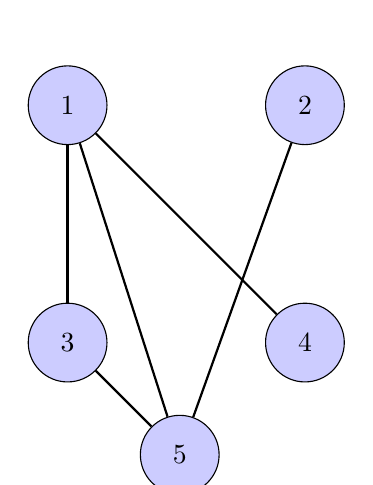
\begin{tikzpicture}
			
			%%
			\begin{scope}[xshift=4cm]
			\node[main node] (1) {$1$};
			\node[main node] (2) [right = 2cm  of 1]  {$2$};
			\node[main node] (3) [below = 2cm  of 1] {$3$};
			\node[main node] (4) [right = 2cm  of 3] {$4$};
			\node[main node] (5) [below right = 1cm  of 3] {$5$};
			
			\path[draw,thick]
			%(1) edge node {} (2)
			(1) edge node {} (3)
			(1) edge node {} (4)
			(1) edge node {} (5)
			%(2) edge node {} (3)
			%(2) edge node {} (4)
			(2) edge node {} (5)
			%(3) edge node {} (4)
			(3) edge node {} (5)
			%(4) edge node {} (5)
			;
			\end{scope}
			\end{tikzpicture}
			
			

\section*{Exercise V}
 For which values of $n$, $r$ is there an $r$-regular graph on $n$ vertices? An
	$r$-regular simple graph?
	
	On $N$ vertices, there is an $r$-regular graph (including multigraphs) if $rn \equiv_2 0$.  \\
	
	if $rn \equiv_2 0$, then at least on of the following is true: $r$ is even or $n$ is even.  \\
	
	In the case where $r$ is even, you can construct an $r$-regular multigraph on $n$ vertices by putting $r/2$ self loops on each vertex.  $2|r$ because $r$ is even, and each self loop increases the degree of the node by $2$ so each node will have a degree of $2$.  \\
	
	In the case where $n$ is even, you can $r$-regular multigraph on $n$ vertices by splitting the graph into pairs.  For each pair, drawn $r$ edges between the vertices.  \\
	
	On simple graphs, it is also possible to construct an $r$ regular graph on $n$ vertices when $rn \equiv_2 0$, with the additional constraint that $n \geq r+1$.  \\
	
	To construct such a graph, relabel the vertices $\in [n]$.  In the case where $r$ is even, draw an edge Each node gets an edge from $r/2$ edges, and has $r/2$ edges drawn from it.  So the graph is $r$-regular.  \\
	
	The construction is similar when $n$ is even and $r$ is odd.  Similarly draw the edges from vertex $x$ to each vertex $y \in [n] $ where $x<y\leq y + \lfloor r/2 \rfloor + 1$ where $+$ is modulo-r arithmetic.  Because $r$ is odd, we must round down and connect to an additional node.  Because it is odd, we will end up drawing the same edge twice.  Ignore this duplicated edge which happens if $n = r + 1$.  

\section*{Exercise VIII}
Suppose that the graph $G-v$ is connected for every vertex $v$ of $G$.
Does it follow that $G$ is connected? (Be comprehensive.)\\

For a graph $G$ where $|V(G)| =1 $, the graph is vacuously connected.  \\ 
For a graph $G$ where $|V(G)| = 2 $, the graph my be connected or may not.  Consider the two ismorphisms on $2$ vertices.  For any $v$, a graph of two vertices which are connected will produce $G-v$ which is always connected, and two vertices which are not connected will produce $G-v$ which is also connected.  \\

By contradiction, I will prove that for any graph $G$ where $|V(G)| > 2$, if $\forall v \in V(G), G-v $ is connected, the graph $G$ is connected.  \\

Assume that we have a graph where $|V(G)| > 2$, if $\forall v \in V(G), G-v $ is connected, but $G$ is not connected.\\
$\implies \exists $distinct $x,y,z \in V(G) $ where there is no path between $x$ and $y$.  \\

The statement of the problem states that $G-z$ will be connected.  If that is true, then there is a path from $x$ to $y$.  By contradiction, any graph $G$ where $|V(G)| > 2$, if $\forall v \in V(G), G-v $ is connected, the graph $G$ is connected.



\end{document}